\chapter{Waveguides}

\section{Introduction}

% EVEREST -> Everest
\begin{figure}[H]
    \centering
    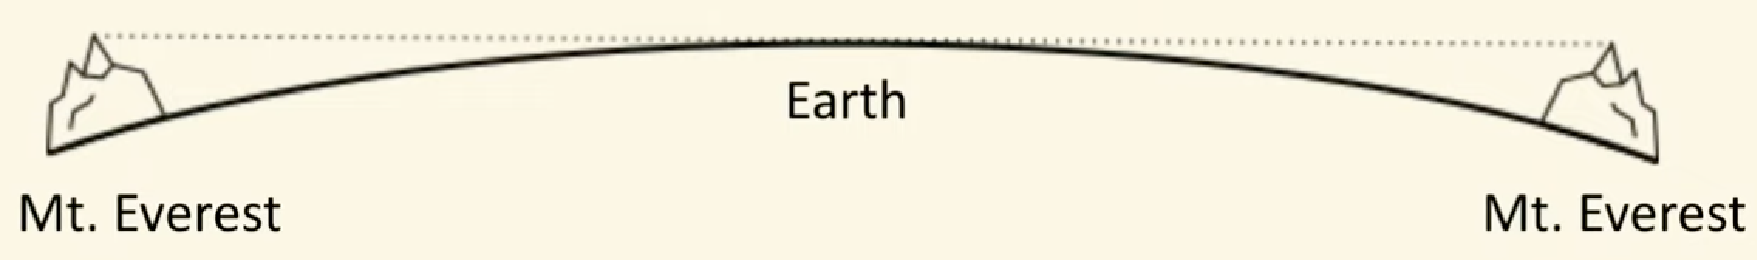
\includegraphics[width=0.9\textwidth]{lesson7/everest.pdf}
    \label{図: 1}
    \caption{The disadvantage of direct transmission of light.}
\end{figure}

Hi, and welcome to Lesson Seven on Wave Guides.

In previous lessons we have talked about how to produce light, whether incoherent or coherent, and then we talked about some properties of coherent light and single photons. Now, we're going to learn how to make wave guides and what are their basic properties.

Step One: Introduction

So let's talk about some of the limitations of unguided light.

One of the properties of light is that it travels very fast, which is actually good because if we encode our message into light, then it means that our message will get to the intended recipient fast. Also, light is fairly unaffected by noise, particularly if it travels in fibers. You can pack many fibers together and they will not be affected by each other's presence, whereas when you compare it to, for example copper cables and transmitting electrical signals, then even the presence of other cables may interfere with your message. Also, light is now relatively easy to produce, but light travels in straight lines, which might sound like a good idea at first, but we will see that actually it's quite limiting in terms of how far we can communicate. So let's consider light traveling in straight lines.

First, of course, there might be some obstacles between the sender and the recipient, so immediately this will make it impossible to reach a recipient.

Then, it's also actually limited to very short range, either because of the first reason that you eventually will hit an obstacle, but also for the fundamental reason that the Earth is curved. So let's do some very quick math. Imagine that this is the surface of the Earth (on slide), and the curvature of course is very much exaggerated here, and let's say that we've got two Mount Everests, so that's the highest point on Earth, and it has a height of just over eight point eight (8.8) kilometers, and let's say that on this Mount Everest (left side), right at the top you place a light source and you are trying to send it to a recipient that's standing on top of the other Mount Everest (right side). So how far can this light travel in a straight line? Well, with some basic trigonometry, actually the distance between Mount Everest one and two is just six hundred seventy two (672) kilometers. So even though it seems like we're very far above the Earth's surface, we cannot really send the light signal that far, and this is discounting any attenuation coming from the atmosphere.

So, being able to guide or steer light seems like a very good idea for long distance communication.

So let's see how it all began. We can say that it began with John Tyndall's experiment. In 1870, what he did was he took a big bucket, filled it with water, and he created a small hole on one side of the bucket at the bottom. And what he noticed was that sunlight that was going into the water was also exiting through this opening in the bucket, but not only that. To his surprise, the sunlight followed the trail that was being taken by the water itself. So the sun rays did not just exit the water bucket in a straight line, but they were being guided by the water itself. So this was one of the first examples of actual fiber, where light was being reflected inside the fiber and guided, and not traveling just in a straight line.

So here's a brief historical outline of the journey that fiber optics have taken. So it all began with in 1870 with John Tyndall's experiment, and people were slowly investigating fiber optics and how to guide light, particularly in glass, but it was only really in 1960 with the invention of laser when people truly realized the potential of using laser light coupled to fiber optics. So they spent a lot of effort in researching how to do that, and in 1966 people managed to couple lasers with fiber optics. And this really sparked the first information revolution. Just to give you some idea how far we've come, in 1970 it was possible to transmit about one percent of the original light over a distance of one kilometer, meaning that if you put in light of some power at the beginning after one kilometer, you only had one hundredth (100th) of the original signal. Twenty years later in 1990, it was possible to transmit ninety six percent (96\%) of the original power over the same distance of one kilometer. And where are we now? In 2021, well, let's have a look at the map of a submarine fiber optic cables. So you can see how many, many cables there are connecting the continents across the Pacific, across the Atlantic, also going from different continents to other continents like this (follow pointer), and this is only the map of the submarine cables. There's a lot more cables going over land, so truly the fiber optic network is the nervous system of mankind, allowing us to communicate within milliseconds from one side of the Earth to the other.

So let's have a quick outline of what we're going to talk about in this lesson. First, we're going to begin with two basic phenomena of how light behaves when it hits the interface of two materials. We're going to talk about reflection and refraction. These two are crucial for understanding how fiber optics works. And then we're going to talk about total internal reflection, where we're going to combine reflection and refraction and derive the condition for total internal reflection. Total internal reflection is what we have seen in Tyndall's experiment, where light was not escaping the water stream but it was being reflected and guided by the water stream. And then we will conclude by some basics of fiber optic cables, in particular how they are constructed and what are the differences between various types of fiber optic cables.


\section{Light at an interface}

Step Two: Light at an Interface

So let's see what happens when a light is trying to go from one medium into a different medium.

Before that, let's see how light can be described.

So light can be viewed as a particle traveling in straight lines, so basically like array. And in order to describe that, all we need is geometric optics. This is the most easiest scenario. Geometric optics relies basically on the laws of trigonometry to describe how the path of light changes as it travels from one medium to the other.

Next step up is if we are interested in the properties of light as a wave, and we've seen this with a double-slit experiment, that light can behave as a wave either when it's a laser light, coherent light, or in the form of single photons, and in order to describe laser light, particularly when it's traveling down a very narrow fibers, we need Maxwell's equations and the full theory of electromagnetism. This description is a lot harder and we're not going to use it here. And finally, the third one is the description of quantum field theory, because light fundamentally is a quantum field. But we're not going to worry about this at all. We're only going to use geometric optics, so the most simple description because mainly we will consider the diameter of the fiber to be much larger than the wavelength of the light, so here "d" is the diameter of the fiber and "lambda" is the wavelength of light, and they give you some ballpark of the numbers that we're going to consider, is d varies somewhere bit from ten, all the way up to two hundred micrometers, whereas the wavelength of light is around of the order of fifteen hundred nanometers (1500nm).

So let's see what happens when the light arrives at an interface of two media.

We're going to consider one medium, usually the air, and then some denser medium, let's say that it's glass. And the light ray is going to arrive at some angle, and this angle will always be measured with respect to the normal to the surface. So we're not going to talk about the angle of incidence as that angle (follow pointer) but the angle between the light ray and then this orthogonal normal line to the surface. So this is the angle of incidence, and we're going to denote it "theta i".

What can happen is that the light can actually reflect off the surface, as this (see pointer), at some angle which we're going to call "theta capital R", the angle of reflection, and also some portion of the light will get refracted, so it will travel into the medium at some angle "theta small r", the angle of refraction. Notice that all of these angles are defined with respect to this dotted line which is the normal to the surface, that's very important.

And often, some portion of the light is reflected, some portion of the light is refracted, and actually it gets transmitted into the other medium. In this case, we're saying that, for example, ninety percent of the light is refracted and enters the glass whereas ten percent gets reflected back. But, we're not going to be too interested in the relationship of how much gets reflected and how much gets refracted, we are more interested in the angles of reflection and angles of refraction. So what is the angle of reflection? Well, that's very simple. The angle of reflection is just the angle of incidence, so "theta i" is equal to "theta R". For example, if we keep increasing the angle of incidence, so we started with this light right here (follow pointer), but then we consider a different light ray, and then a different one, all with different angles of incidence, the corresponding angles of reflection are also increasing.

Now, let's talk about angle of refraction. This is going to be a little bit more complicated. As you can see from this image here, the angle of incidence and angle of refraction are different. So let's see how we can actually compute them, and for that, we need something called refractive index of a material.

Refractive index is defined as follows: we're going to denote it as "n", and it's given as "c over v". So n, we said, is the refractive index, c is the speed of light in vacuum, and v is the speed of light in the medium. So really, what refractive index tells us is how much does the speed of light change in this new medium. For example, this refractive index of vacuum is just one. Why? Because in vacuum, the light travels with the same speed c, so c over c is equal to one. Air has a slightly larger refractive index, but for our purposes it's basically just one, so the speed of light does not change very much, it slows down a little bit but very very small amount. Glass on the other hand, has a refractive index of 1.46 (one point four six), so it means that the light travels 1.46 times slower in the glass than when we compare it with the speed of light in vacuum. And in diamond, it travels even slower by a factor of 2.42 (two point four two), which is the refractive index of diamond.

So let's get back to our example of light ray being incident on a surface.

So, we're going to denote the refractive index of the top medium as n-i. "i" stands for anything that's incident onto the surface. And n-r is the refractive index of the material into which the light ray transmits and gets refracted. And the angles follow this relationship (eq. on top right), so the sine of the incidence angle, divided by the speed of light in that medium, is equal to the sine of the refracted angle theta R, over the speed of light in the new medium. So we can use this relationship between the refractive index and the speed of light in the medium, and we just substitute for v-i, and we substitute for v-r, and we obtain the following relationship: it's n-i times sin(theta i), is equal to n-r sin(theta r). So the refractive index of the medium on top here (n-i), times the sine of the incidence angle theta i, is equal to the product of the refractive index of the new medium and times the sine of angle of refraction. And this is known as "Snell's law", and this law is very useful and we're going to use it extensively in this and following lessons.

So, before we do any computations, let's see what actually happens with the angles as light travels from, let's say a less dense medium into a more dense medium. So what that means is that n-i is smaller than n-r. For example, if we are considering the example of light traveling in air and then trying to move into glass. Again, substituting into our Snell's law and rearranging a little bit, we've got n-i over n-r, so we brought this n-r on to the other side (LHS), and then we also divided by sine theta i, so we've got that the fraction of n-i over n-r, has to be equal to sine theta r over sine theta i. And from our assumption that we are traveling from less dense medium into more dense medium, we can see that the fraction of the left-hand side is smaller than one. What this means that this fraction over here (RHS) also has to be smaller than one, and that's achieved when theta r is smaller than theta i, meaning that the angle of refraction is smaller than the angle of incidence. So we see that when light travels from a less dense medium into more dense medium, it bends towards the normal. Now, what happens in the opposite scenario when we are traveling from a more dense medium into a less dense medium? Well, we can go through the same calculation again, but this time we assume that n-i is larger than n-r, and we substitute it in. We see that the ratio on the left hand side of n-i over n-r is larger than one, therefore we conclude that the angle of refraction has to be larger than the angle of incidence, so if we are going from a more dense medium into a less dense medium, we are refracting away from the normal.



\section{Total internal reflection}

Step Three: Total Internal Reflection

In the previous step, we have seen that if light is incident on a surface and traveling from a more dense medium into a less dense medium, then it gets bent away from the normal axis. The angle of refraction, so this angle over here (see pointer), is larger than the angle of incidence. So we can have the scenario where we are increasing steadily the angle of incidence, and the refracted beam of light is being bent further and further away from the normal axis that's perpendicular to the surface of the material. So we can ask the question: is there such an angle of incidence where the refracted beam travels parallel to the surface to the interface between the two media? Meaning, we are looking for a scenario where the angle of refraction is ninety degrees, and yes, there is. So we are looking for this scenario (see slide), we have our incident beam hitting the interface between glass and air at such an angle such that the refracted beam travels at ninety degrees to the normal or parallel to the surface between air and glass. So let's now compute this angle using Snell's law.

We have that the n-i, the refractive index of glass, times the sine of the angle of incidence, is equal to the refractive index of air n-r, times the sine of theta r, but we know that here we are looking for a scenario where the sine of theta r is just sine of ninety degrees which is equal to one. So we have the following relationship (see pointer), and we have changed the subscript here on this theta to "theta c" which stands for "critical angle", because that's the critical angle where we obtain angle of refraction of ninety degrees. Now we can just rearrange to get sine of theta c, equal to as a simple fraction of n-r over n-i. In our case, here n-r is the refractive index of air and n-i is the refractive index of glass, and we can just take the arc sine ($\sin^{-1}$) to obtain this expression for the critical angle. When this happens, then we said that the light ray travels parallel to the surface, but we can also keep increasing the angle of incidence to theta i being larger than the critical angle theta c, and in that case what happens, we get "total internal reflection", so the light ray comes in and gets totally reflected back to inside the glass, and this is the case that we saw in the first step of Tyndall's experiment where the light was being internally reflected and guided by the stream of water.

So let's consider some numerical examples: here we are keeping the refractive index of the outside medium, which for us is air, fixed. So it's just 1.00028, it's basically the same as one. And what we are changing is the material of the fiber, so we are changing the refractive index of n-i, and we are looking at the value of the critical angle beyond which total internal reflection can occur. So if we are plotting the arc sine of the previous expression for the theta c, then we get the following curve (see slide). So we see that as we are increasing the density of the material, we are decreasing the critical angle beyond which we get total internal reflection. For example if we look at the interface of water and air, water has a refractive index of 1.33, so that's this line over here, and we obtain a critical angle of around fifty degrees. Glass is a little bit more dense than water, it has refractive index of 1.46 and the angle of the critical angle beyond which we get total internal reflection is a little bit smaller than the water, and for diamond which has a very large refractive index of 2.42, then the angle is slightly over twenty degrees. So what does all this means, that the critical angle is decreasing? Well, it means that in glass, if we want to obtain total internal reflection, then the angle of incidence, which again I remind you is the angle between the incident light ray and the normal to the surface, has to be large, meaning that the angle between the surface- so measured with respect to the interface between air and glass, has to be quite small, then we get total internal reflection. Whereas in diamond, the light is confined more strongly, it can have a incident angle which is smaller than it is in the glass, so even if it's incident on the surface at this much steeper angle, it still can get reflected and be contained and guided by the fiber.



\section{Optical fibers}

Step Four: Optical Fibers

Let's have a look at what a typical optical fiber consists of.

On the outer layer, we've got the jacket, and this is to protect the inside components of the fiber. The next in line is the buffer. Now the buffer is there also for protection, but it can also bundle multiple optical fibers.

Then we've got the cladding over here, and this is the material that is responsible for reflecting light back and keeping it contained within the inside, which is the core. Also, cladding serves as a form of protection and prevents crosstalk, because if you have two cores next to each other, then light can easily escape to the other core, so you must separate them somehow and that's the purpose of the cladding. So these two components (cladding and core) are the ones that are optically important parts. Core is the one that carries the light signal and it has some refractive index n-f, "f" for fiber, whereas cladding has a smaller refractive index n-c, and that's the one that is responsible for reflecting light back into the core and keeping it constrained inside the fiber. And there are two main types of fibers. One is the "multimode fiber", over here (see slide), so you can see that here the modes are represented by different spatial beams bouncing inside the fiber, and "single mode fibers" which are so narrow that there's only one mode permitted to travel inside the fiber.

So let's look at multi-mode fibers first. As we said, here all of these rays (see slide), they represent various modes of light traveling inside the fiber, and what's important for multi-mode fibers is the angle of acceptance. This is the angle represented by this gray cone over here, and if the light comes traveling inside the fiber within this light cone, then it will couple to the fiber and undergo many internal reflections inside the fiber, and basically be carried inside and be guided by the fiber. But, if the incident angle of the light is such that it is outside of the acceptance cone, then it will just hit the cladding and get refracted outside and get absorbed, so it will not be coupled to the fiber. So, let's apply Snell's law and actually calculate what is the maximum permissible permitted angle such that we couple to the fiber.

So we have the following scenario: in here we actually have two interfaces. One interface is the usual between the fiber with refractive index n-f, and the cladding with refractive index n-c, but now we also have to consider the light coming into the fiber, so we also consider refractive index of some material that's outside of the fiber and we will denote it by n-i. And we've got these three angles (see slide). We are looking for the maximum theta- maximum permitted angle, and if we multiply it by two, this is called the acceptance angle. And we want this angle to be such that when the light gets refracted into the fiber and then hits the cladding, it gets reflected completely and totally back into inside the fiber. So this angle, we set to theta c, which is the critical angle needed for total internal reflection. Using basic trigonometry, then we know that this angle of refraction at the surface of the fiber and whatever material is outside of the fiber has to be ninety degrees minus theta c.

And we all know from previous step that if we take the sine of this critical angle, so this angle over here (see pointer), it has to be equal to the ratio of the refractive indices of the cladding and the fiber, so sine theta c is equal to n-c over n-f.

Then we continue using our Snell's law, so at this interface between the fiber and the outside material (see pointer), we write that n-i, the refractive index of the outside material, times sine theta max, has to be equal to the refractive index of the fiber times sin(ninety degrees minus theta c), which is the angle of refraction over here measured with respect to the normal of the surface, which in this case is given by this horizontal dashed line.

And we can simplify using trigonometric identity, sin(ninety degrees minus theta c) is just equal to the cosine of that angle theta c, and we can use another trigonometric identity where we use the fact that sine squared of an angle plus the cosine squared of the angle has to be equal to one. So cosine of theta c is just equal to one minus sine squared theta c, the whole expression square rooted.

And using the expression that we have over here for the critical angle (see pointer), we can just substitute an expression for sine squared theta c, which is just n-c squared over n-f squared.

So finally, we have the following expression: multiplying this (see pointer) by n-f, we get that the n-i times sine theta max, is equal to the square root of n-f squared minus n-c squared, and this gives us the "theta max", the maximum angle of acceptance and therefore also, the cone of acceptance.

And this number on the left hand side, this product of the refractive index times the max sine of the maximum acceptance angle, is known as numerical aperture, and the higher the numerical aperture is, the better we can couple to the fiber, meaning that this incident angle over here which we are calling theta max, is allowed to be larger.

So, what are some properties of multi-mode fibers? Well, we said that their diameter is much larger than the wavelength of the light, and typically they've got diameters larger than ten micrometers, and they can go up to something like two hundred micrometers. So we said, in order to describe their behavior, it is enough to consider light traveling as a particle traveling in straight lines, and using basic trigonometry, so we can use geometric optics which we have been doing so far in order to derive some useful properties of the multimode fiber.

Second, the light inside travels at different angles, meaning that it can carry multiple modes at the same time.

But, what this causes, is because the path lengths of the various parts- of the various light rays differ, we get mode dispersion, and we will describe that in a later lesson and look at it more closely. And such a fiber, because of mode dispersion, is more suited for short distances, so meaning inside office networks or campus networks. And also, it is relatively cheap to manufacture, mainly because it's quite thick. On the other hand, a single mode fiber can carry only a single mode of light, so there's only one ray traveling in one direction like this (follow pointer).

And now, the diameter is typically smaller than ten micrometers, and just to give you an idea how thin that is, the human hair is usually larger than twenty micrometers. There's a large variance, but it's between twenty, and perhaps two hundred micrometers, so they're extremely extremely thin. And because they are so thin, it is no longer possible to describe them using geometric optics. We have to resort to using electromagnetic theory and Maxwell's equations. But, because they are so thin and there's only a single mode, there is no mode dispersion and that is why they allow for very high rate of transfer of data, and therefore they are suitable for long distance communications. They have to be boosted by repeaters approximately every fifty kilometers, but we will see how that can be achieved in a later lesson. But because they are so thin, they are quite expensive to produce.

And a small, small note at the end: the first transatlantic fiber optic cable, which was called TAT-8, was laid in 1988 between Tuckerton, New Jersey, and then it traveled across the Atlantic and then split into the UK and France and it was constructed at a cost of approximately 335 million US dollars, and it was retired in 2002. So it was predicted that the bandwidth of this fiber optic cable would last for a long time and perhaps never be reached. The bandwidth was two hundred eighty megabits per second (280 Mbits/s), which can carry around forty thousand phone circuits simultaneously, and this capacity was reached in eighteen months. Now this just demonstrates how quickly how quickly we can consume data, and how quickly we need to transfer data and the size of the data that we need to transfer.



\newpage
\begin{exercises}
\exer{Consider the following quantum state:}
\begin{equation*}
\ket{\psi} = \frac{\sqrt{3}}{2}\ket{0} + \frac{1}{2}\ket{1}
\end{equation*}
\subexer{Find the probability of measuring a zero.}
\subexer{Find the probability of measuring a one.}


\end{exercises}

\newpage
\section{Quiz}

\section{Further reading Lessons 5-7}

Lesson 5

This Lesson discusses the various types of light depending on their coherence properties. Coherent light produced by lasers is crucially important from the perspective of communication. A good qualitative as well as quantitative introduction to lasers can be found in Chapter 1 of:

Orazio Svelto, Principles of Lasers, Springer, 2009.

A great discussion of lasing behaviour from the perspective of a mathematician (but still explained very intuitively) is in Chapter 3 of the classic:

Steven H. Strogatz, Nonlinear Dynamics and Chaos: With Applications to Physics, Biology, Chemistry, and Engineering, CRC Press, 2000.

Lesson 6

Two great optics textbooks for this Block as well as the following ones are:

Eugene Hecht, Optics, Pearson, 2015.
Grant R. Fowles, Introduction to Modern Optics, Dover Publications, 1989.
Bahaa E. A. Saleh, Malvin C. Twitch, Fundamentals of Photonics, Wiley-Interscience, 2007.

These books focus on wave and geometric optics and provide a good foundation for transitioning to quantum optics which we will do later.

Interference is an extremely important concept we encourage you to read and understand the discussion in Chapter 1 in:

Richard P. Feynman, Robert P. Leighton, Matthew Sands, The Feynman Lectures on Physics, Vol. 3, Addison Wesley, 1971.

Lesson 7

This Lesson relies mainly on the geometric description of light propagation. Section 4.3 and Section 5.6 of Hecht’s textbook contain great discussion of reflection and propagation in optical fibers, respectively.
